\documentclass[a4paper, 11pt]{article}
%\usepackage[round]{natbib}

\usepackage{mathtools}
\usepackage{setspace} 
\usepackage{dsfont}
\usepackage{amsfonts}
\usepackage{amsmath}
\usepackage{subcaption}
\usepackage{paralist}
%\usepackage{subfig}
\usepackage{times}
\usepackage{latexsym}
\usepackage{graphicx}
\usepackage[T1]{fontenc}
\usepackage{tikz}
\usepackage{tikz-qtree}
\usetikzlibrary{positioning}
\usepackage{url}
\usepackage{pgfplotstable}
\usepackage{titlesec}
\usepackage{color}
\usepackage{lipsum,adjustbox}
\usepackage[font={small}]{caption}

\usepackage{bbm}

\makeatletter
\newcommand{\@BIBLABEL}{\@emptybiblabel}
\newcommand{\@emptybiblabel}[1]{}
%\makeatother
\usepackage[draft,	hidelinks]{hyperref}


\usepackage{naaclhlt2018}
\graphicspath{{./plots/}}
\newcommand{\com}[1]{}
%\newcommand{\oa\part{title}}[1]{}
%\newcommand{\lc}[1]{}
\newcommand{\oa}[1]{\footnote{\color{red}OA: #1}}
\newcommand{\oamod}[1]{{\color{red}#1}}
\newcommand{\lc}[1]{\footnote{\color{blue}LC: #1}}
\newcommand{\lcmod}[1]{{\color{blue}#1}}

\newenvironment{myequation}{
  \vspace{-1em}
 \begin{equation}
}{
 \end{equation}
 \vspace{-1.2em}
}
\newenvironment{myequation*}{
	\vspace{-1em}
	\begin{equation*}
}{
\end{equation*}
\vspace{-1.2em}
}


\begin{document}

\title{Reference-less Measure of Faithfulness for Grammatical Error Correction}
%\author{
%  Leshem Choshen\textsuperscript{1} and Omri Abend\textsuperscript{2} \\
%  \textsuperscript{1}School of Computer Science and Engineering,
%  \textsuperscript{2} Department of Cognitive Sciences \\
%  The Hebrew University of Jerusalem \\
%  \texttt{leshem.choshen@mail.huji.ac.il, oabend@cs.huji.ac.il}\\
%}
\maketitle

\begin{abstract}
  We propose {\sc USim}, a semantic measure for Grammatical Error Correction (GEC)
  that measures the semantic faithfulness of the output to the source,
  thereby complementing existing reference-less measures (RLMs) for measuring the output's grammaticality.
  {\sc USim} operates by comparing the semantic symbolic structure of the source and the correction,
	without relying on manually-curated references.
  Our experiments establish the validity of {\sc USim},
  by showing that the semantic structures can be consistently applied to ungrammatical text, that
  valid corrections obtain a high {\sc USim} similarity score to the source, and that
  invalid corrections obtain a lower score. 
  %grammatical reference-less evaluation measure to
  %create a measure balancing between the goal of correcting grammatical mistakes and the goal of
  %conveying the original meaning.
\end{abstract}


%%%%%%%%%%%%%%%%%%%%%%%%%%%%%%%%%%%%%%%%%%%%%%%%%%%%%%%
\section{Introduction}

Evaluation in Monolingual Translation, and in Grammatical Error Correction (GEC) is a challenging
research field, much due to the difficulty in integrating 
different types of rewriting operations into a single measure, and the vast number of valid outputs
\cite{tetreault2008native,madnani2011they,chodorow2012problems,bryant2015far}.
These difficulties, as well as the idiosyncrasies of GEC have recently motivated
a number of proposals for new, improved reference-based measures (RBMs)  \cite{dahlmeier2012better,felice2015towards,napoles2015ground}.

Nevertheless, the size and heterogeneity of the space of valid outputs per sentence often prohibits
obtaining a reference set that covers this space well, thereby limiting the applicability
of RBMs \cite{bryant2015far}.
To address this we propose a semantic RLM, {\sc USim}.
{\sc USim} operates by measuring the graph distance between the semantic
representations of the source and the output.

Our proposal complements the RLM proposed recently by 
\newcite{napoles-sakaguchi-tetreault:2016:EMNLP2016}, which uses grammatical error detection techniques to assess the grammaticality of the output.
A similar decomposition of output quality to its adequacy (similar to faithfulness)
and fluency (related to grammaticality), has been used in machine translation(MT)
evaluation \cite[e.g.,][]{banchs2015adequacy}.

As a test case, we use UCCA semantic representation \cite{abend2013universal},
motivated by its recent use in semantic MT evaluation \cite{birch2016hume}.
However, the measure can be easily adapted to use other semantic schemes, e.g., AMR \cite{banarescu-EtAl:2013:LAW7-ID}.

{\sc USim} is conceptually related to RLMs developed
for MT
\cite{reeder2006measuring,albrecht2007regression,specia2009estimating,specia2010machine}.
Notably, XMEANT \cite{lo2014xmeant} compares the source to the output
in terms of their semantic role labeling structures.
Our use of UCCA is motivated by its wider coverage of predicate types, as opposed to 
MEANT's focus on verbal argument structures, and its subsequent preservation
of structure across translations \cite{sulem2015conceptual}.
See \cite{birch2016hume} for a more elaborate comparison. 

%{\sc USim} allows changes to the source, but only to the extent that these changes
%do not alter the semantic structure. 

%We show that due to the vast number of possible valid corrections, reference-based measures suffer from 
%biases that will not be solved by more references. 
%Specifically, systems developed towards such measures 
%hardly correct, state-of-the-art systems are such systems. 

%Semantic annotation schemes are also gaining support and proven to be useful for many tasks in general\lc{have preference on what to cite?} and specifically for evaluation \cite{birch2016hume}. One desired feature of semantic annotation is its robustness to modifications that do not change the meaning such as paraphrasing \cite{abend2013universal}, and translation \cite{sulem2015conceptual}.

We conduct experiments to confirm the {\sc USim} validity.
Specifically, we show
(1) UCCA can be consistently and automatically applied to learner language (LL), 
(2) {\sc USim} is not prone to unduly penalize valid corrections, and 
(3) {\sc USim} assigns a lower score to corrections of poor quality.
Our experiments also indicate that UCCA parsing technology is already sufficiently mature for an automatic variant of {\sc USim} to provide reliable results.
\vspace{-.6cm}

\section{Background}
\vspace{-.1cm}

\paragraph{Structural Annotation of Learner Language.}
While linguistic theories propose that each learner makes consistent use of syntax 
\cite{huebner1985system,tarone1983variability}, this use may not conform to the syntax of the learned language, 
or of any other known language. This entails difficulties in defining syntactic annotation for LL, as the syntax annotated differs for each learner.

Syntactic schemes for LL annotate syntactically erroneous sentences in different ways.
\newcite{berzak2016universal} and \newcite{ragheb2012defining} annotate according 
to the syntax used by the learner, even if this use is not grammatical.
Such annotation may be unreliable as a source of semantic information, 
as GEC systems aim to alter these erroneous syntactic structures.
\newcite{nagataphrase} take the opposite approach, and remain faithful to the syntax intended by the learner.
This has also been the tradition in works on parser robustness 
\cite{bigert2005unsupervised,foster2004parsing}. However, such approach is prone to inconsistencies due to the 
variety of different syntactic structures that can be used to express a similar meaning. 

In this paper, we use semantic annotation to structurally
represent LL text. Semantic structures are faithful to the intended
meaning of the sentence, and not to its formal realization, and thus face
fewer conflicts where the syntactic structure used diverges from
the one intended. We are not aware of any previous attempts to semantically
annotate LL text.

\vspace{-.2cm}
\paragraph{The UCCA Scheme.}\label{sec:ucca}
UCCA is a semantic annotation scheme that builds on
typological and cognitive linguistic theories.
The scheme's aims are to provide a coarse-grained, cross-linguistically
applicable representation.
Importantly, UCCA's categories directly reflect semantic, rather than
distributional distinctions.
For instance, UCCA is not sensitive to POS distinctions:
a Scene's main relation can be a verb but also an adjective
(``He is {\bf thin}'') or a noun (``John's {\bf decision}'').
Indeed, \newcite{sulem2015conceptual} have found that UCCA structures are
preserved remarkably well across English-French translations. 

UCCA structures are directed acyclic graphs, where the words in the text 
correspond to (a sub-set of) their leaves.
The nodes of the graphs, called {\it units}, are either leaves or several elements jointly
viewed as a single entity according to some semantic or cognitive consideration.
The edges bear one or more categories, indicating the role of 
the sub-unit in the relation that the parent represents.

UCCA views the text as a collection of {\it Scenes} and relations between them.
A Scene describes a movement, 
an action or a state which is persistent in time.
Every Scene contains one main relation, 
zero or more {\it Participants}, 
which are interpreted in a broad sense, 
and include locations, destinations and complement clauses,
and {\it Adverbials}, such manner descriptions.

\com{
\begin{figure}[t]
				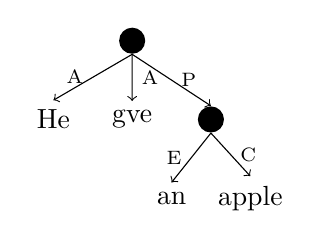
\begin{tikzpicture}[sibling distance=10mm, level distance=10mm, ->,
				every node/.append style={midway},
				every circle node/.append style={fill=black}]
				{
					\node (Source) [circle] {}
					child {node (He) {He} edge from parent node[left] {\scriptsize A}
					}
					child {node (gave) {gve} edge from parent node[right] {\scriptsize A}}
					child {node (an apple) [circle] {}
						{
							child {node (an) {an} edge from parent node[left] {\scriptsize E}}
							child {node (apple){apple} edge from parent node[right] {\scriptsize C}}
						} edge from parent node[right] {\scriptsize P} }
					;}
					\end{tikzpicture}

		\end{figure}}
		
\section{Semantic Faithfulness Measures}\label{sec:Semantics}
\begin{figure}[t]
		\hspace{-1.3cm}
		\begin{subfigure}{1.1\columnwidth}
			\vspace{-0.2cm}
			\parbox{.8\columnwidth}{\hspace{1cm}
				\scalebox{.9}{
					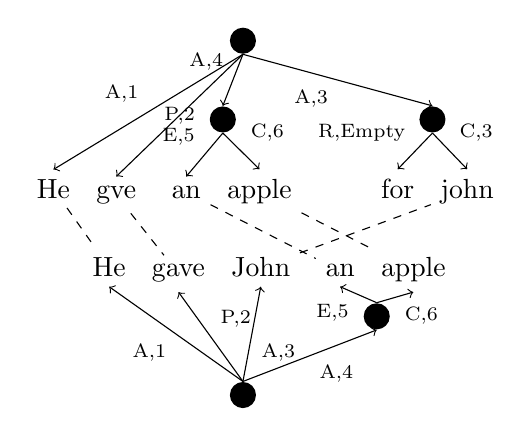
\begin{tikzpicture}[sibling distance=1mm, level distance=10mm,
					every node/.append style={midway},
					every circle node/.append style={fill=black}]
					\begin{scope}[frontier/.style={distance from root=20mm}, ->]
					\Tree [.\node [circle] (rootu) {};
					\edge node [auto=right]{\scriptsize A,1}; \node (Heu) {He};
					\edge node[auto=right down]{\scriptsize P,2}; \node (gve) {gve};
					\edge node[auto=right]{\scriptsize A,4};
					[.\node [circle](an appleu) {};
						\edge node[auto=right]{\scriptsize E,5}; \node (anu) {an};
						\edge node[auto=left]{\scriptsize C,6}; \node (appleu) {apple};
					]
					\edge node[auto=right]{\scriptsize A,3};
					[.\node [circle](for john) {};
					\edge node[auto=right]{\scriptsize R,Empty};\node (for) {for};
					\edge node[auto=left]{\scriptsize C,3}; \node (john) {john};
					]]
					\end{scope}
					\begin{scope}[yshift=-4.5cm,grow'=up, frontier/.style={distance from root=15mm}, ->]
					\Tree [.\node [circle] (rootd) {};
					\edge node [auto=left]{\scriptsize A,1}; \node (Hed) {He};
					\edge node[auto=right]{\scriptsize P,2}; \node (gave) {gave};
					\edge node[auto=right]{\scriptsize A,3};\node (John) {John};
					\edge node[auto=right]{\scriptsize A,4};
					[.\node [circle] (an appled) {};
					\edge node[auto=left]{\scriptsize E,5}; \node (and) {an};
					\edge node[auto=right]{\scriptsize C,6}; \node (appled) {apple};
					]
]
					\end{scope}
					\begin{scope}[dashed]
					\draw (Heu) -- (Hed);
					\draw (gve) -- (gave);
					\draw (John) -- (john);
					\draw (anu) -- (and);
					\draw (appleu) -- (appled);
					\end{scope}
					\end{tikzpicture}
				}}
				\parbox{.1\columnwidth}{
					\vspace{2cm}
					\begin{adjustbox}{width=.3\columnwidth,margin=1pt,frame}
						\begin{tabular}{ll}
							A & participant \\
							H & linked scene \\
							R & relator \\
							C & center \\
							E & elaborator \\
						\end{tabular}
					\end{adjustbox}
				}
			\end{subfigure}

				\caption{\label{fig:example}
					UCCA structures of a learner language (top) and correction (bottom) including word alignments (dashed). On the edges are labels and numbers aligned to (top) or indexes (bottom). Precision is $\frac{7}{9}$ Recall is $\frac{7}{7}$.
				}
			\end{figure}
We start by defining a simplified measure that compares two UCCA annotations over the 
same set of tokens, which is used to measure inter-annotator agreement (IAA). We then
proceed to defining {\sc USim}, which compares two UCCA structures
over alignable but different sets of tokens.

\paragraph{IAA Measure.} We define a similarity measure over UCCA annotations 
$G_1$ and $G_2$ that share their set of leaves (tokens) $W$.
For a node $v$ in $G_1$ or $G_2$, define its yield $yield(v) \subseteq W$ as its
set of leaf descendants.
Define a pair of edges $(v_1,u_1) \in G_1$ and $(v_2,u_2) \in G_2$ to be matching
if $yield(u_1) = yield(u_2)$ and they have the same label.
Labeled precision and recall are defined by dividing the number of matching edges
in $G_1$ and $G_2$ by $|E_1|$ and $|E_2|$ respectively.
{\it DAG $F$-score} is their harmonic mean.
The measure collapses to the common parsing $F$-score if $G_1, G_2$ are trees.

\paragraph{The {\sc USim} Measure.} Computing a faithfulness
measure is slightly more involved, as the source sentence graph $G_s$ and its
correction $G_c$ do not share the same set of leaves.
%Giving a more accurate
%measure than the upper bound suggested by \cite{sulem2015conceptual} for
%comparing two parallel texts in different languages, while keeping
%the essence of comparing how many of the aligned nodes conserve meaning and tag. For that we may think for a moment on GEC as
%translation from LL to Proper English, and a good translation
%would be a translation which keeps the meaning but has the syntax
%of English. Considering that, just like in translation, we can align words from the LL to the corresponding words in English
%and keep record of how many of those nodes kept their labels.
%
%As comparing labels is trivial, and done before us. We should focus on how we propose to align nodes. 
%First, note that comparison should not be at
%the token level, as we want to allow tokens to be corrected - replaced or removed -
%as long as the higher structures convey the same meaning. We thus
%prune the s above the leaves, the tokens of the sentence. To
%define an alignment of the nodes, we suggest some possible ways, all
%based on first aligning the words in order to give order to the DAG and then comparing the structure in one way or another.
%
We assume a (possibly partial, possibly many-to-1) alignment between $G_s$ and $G_c$,
$A \subset V_s \times V_c$. 

An edge $(v_1,v_2) \in E_c$ is said to match an edge
$(u_1,u_2) \in E_s$ if they have the same label and $(v_2,u_2) \in A$. Recall (Precision)
is defined as the ratio of edges in $E_s$ ($E_c$) that have a match in $E_c$ ($E_s$) respectively, and
$F$-score is their harmonic mean. We note that this measure collapses to the
{\it DAG $F$-score} if $A$ includes all pairs of nodes in $E_s$ and $E_c$ that have
the same yield. See Figure \ref{fig:example}. 

In order to define the alignment between $V_s$ and $V_c$, we begin by aligning the leaves
(tokens) in $V_s$ and $V_c$.
We cast alignment as a weighted bipartite graph matching problem. Edge weights are assigned to be the edit distances between the tokens.
We note that aligning words in GEC (and other monolingual translation tasks) is much simpler than in MT,
as most of the words are unchanged, deleted fully, added, or changed slightly.
Denote the resulting leaf alignment with $A_l \subset Leaves_s \times Leaves_c$.
We now extend $A_l$ to define the node alignment $A$, aligning each non-leaf $v \in V_s$
with the node $u \in V_c$ that maximizes

\begin{small}
	\vspace{0.15cm}
 \begin{myequation*}
  w\left(v,u\right) = \frac{\vert A_l \cap \left(yield\left(u\right) \times yield\left(v\right)\right)\vert}{\vert yield\left(u\right) \vert}.
 \end{myequation*}
 %\vspace{0.1cm}
\end{small}

We exclude from $A$ zero weighted pairs.
The resulting $F$-score measure, using the resulting $A$ is called UCCA Similarity ({\sc USim}).
As the resulting alignment may differ when aligning nodes from $V_c$ to $V_s$
and the other way around, we report the resulting $F$-score in both directions.

Note that {\sc USim} is somewhat more relaxed than {\it DAG $F$-score},
as it also aligns nodes whose yields are not in valid alignment with one another,
unlike DAG $F$-score which requires a valid match.
While this relaxation is necessary, given that corrections often add
or remove nodes, thus eliminating the possibility of a valid alignment,
in order to obtain comparable IAA scores, we report IAA using {\sc USim} as well.
%
%Then for each node in $v \in V_s$, we compute its descendent leaves $yield(v) \subset Leaves_s$ as before,
%and compute their projection $yield'(v) = \{u \in Leaves_c:(v,u) \in A_l\}$.
%We now define the node alignment to be $A = \{(u,v) \in V_s \times V_c : yield'(u) = yield(v) \}$.
%We note that $A_l \subset A$ and that if $V_s$ and $V_c$ share the same tokens,
%this computation again reduces to DAG $F$-score.

For completeness, we replicate the protocol used by \newcite{sulem2015conceptual}
for comparing the UCCA annotations of standard English-French translations, which we call
Distributional Similarity ({\sc DistSim}).
For a given UCCA label $l$, $c_i(l)$ is the number of $l$-labeled UCCA edges
in the i-th source sentence, and $d_i(l)$ is the number of $l$-labeled UCCA edges
in its corresponding correction. We define {\sc DistSim}(l) between these
sentences to be $\frac{1}{N}\sum_{i=1}^N \vert c_i(l) - d_i(l) \vert$, where
$N$ is the total number of sentence pairs.

%
%A first and most straightforward approach would be to compare all
%pairs of nodes in parallel paragraphs and to each node from one paragraph
%assign the one most similar node, span wise from the other. That approach
%is quite similar to the IAA aligning, but it
%has three drawbacks; it is asymmetric; it may be over optimistic aligning
%nodes without considering the DAG structure; and it might be
%slow for many nodes. Being asymmetric is not much of a problem. If we thrive for symmetry
%we can compute the measure twice and use the results mean,
%that would also be the case for other asymmetric methods we suggest.
%In order to address the other drawbacks we propose different aligning methods.
%
%A second method driven by the assumption that nodes higher in the
%hierarchy are more important to the semantic representation is measuring
%the largest cut in which nodes are aligned (top down) to each other
%and have the same labels. This is a harsher lower similarity
%score but one of which might be more representative of the semantics
%that are kept and hopefully more informative for tasks that will use it.
%
%A third type of methods were token similarity methods, these methods
%use one kind of aligning (top down, bottom up or pairwise) and only
%compare the meaningful nodes. This was called upon by \cite{sulem2015conceptual}. 
%This approach makes sense due to the fact that some labels
%are well defined and thought upon while others are still vague and
%call for future work on refining or adjusting them, moreover, some
%labels are more semantic while other labels are currently just a place
%holder as each node must get a level, and the semantic role is not
%always clearly defined (e.g., the word ``is'' in ``he is walking''
%seem to be more syntactically related than semantically. In UCCA it is tagged as a \textit{function} word.). The unused
%labels are center, elaborator, function, relation, linker, ground
%and connector.
%
%A bit different way than all the others is to compute the labeled
%tree edit distance\cite{zhang1989simple}, for that we first needed
%the trees to be ordered, we did that in a top down fashion. An interesting
%future work would be to use unordered tree edit distance methods\cite{zhang1992editing}.
%
%We see that measurements for symmetry that are similar to the inter
%annotator agreement measure also suggest high stability, achieving
%scores not much lower than the one different annotators get for the
%same paragraph. This result is quite strong as an inter annotator
%agreement is the upper bound being the score of comparing a paragraph to itself. 
%Most importantly we learn from it all that even when correcting grammatical errors,
%the semantic structure (as represented by UCCA at least) is hardly changed and thus
%can be used as a tool to avoid introducing semantic changes when trying to only change grammar. 
%The symmetry measures we introduce can be used to enforce semantic conservatism.
%In conclusion, we have shown some direct ways to measure
%semantic faithfulness. Such ways will allow correctors to be less formally conservative
%while controlling semantic conservatism. Thus, focusing on what users - and hence we - are more interested in.
%
%
\vspace{-.2cm}
\section{Experiments}
\vspace{-.2cm}


We conduct four types of experiments to validate the feasibility of our approach.
First, we show that semantic annotation can be consistently applied to 
LL, through inter annotator agreement (IAA) experiments.
Second, we show that a valid corrector scores high on this measure.
Third, we show an automatic UCCA parser can reliably replace human annotation in {\sc USim}.
Fourth, we show that {\sc USim} is sensitive to changes in meaning, 
by comparing the semantic structures of the source to corrections of fairly poor quality.

\vspace{-.2cm}
\paragraph{Experimental Setup.}
We train two UCCA annotators by annotating both LL and standard English
passages, until a high enough agreement has been reached (a total of 6 hours of training).
Training passages are excluded from the evaluation.
We use UCCA's annotation
guidelines\footnote{\url{http://www.cs.huji.ac.il/~oabend/ucca.html}}
without any adaptations.

We experiment on 7 essays and their corrections, each comprising about 500 tokens.
In order to measure IAA, we assigned 4 of these essays to both annotators
and compute their agreement.
In order to measure the faithfulness score for a valid correction,
we annotate both the source
and the manually corrected versions of 6 essays,
3 of which were annotated by both annotators.

\vspace{-.2cm}
\paragraph{The Faithfulness of Valid Corrections.}
We obtain an IAA {\it DAG $F$-score} of 0.845
(Precision 0.834, Recall 0.857), which
is comparable to the IAA reported for English Wikipedia texts by \cite{abend2013universal}.
As another point of comparison, we doubly annotate 3 corrected
NUCLE \cite{dahlmeier2013building} passages, obtaining a similar IAA.
These results suggest UCCA annotating LL does not degrade IAA, 
it can be applied as consistently to LL as to standard English.

Table \ref{tab:Distances} (left-hand side) presents the {\sc USim} scores obtained by comparing 
the NUCLE references and the source, or equivalently the score of a valid correction.
To control for differences between the annotators, we explore both
a setting where both sides are annotated by the same annotator,
and a setting where they are annotated by different ones.
As an upper bound on the score of a valid corrector (using different annotators),
we also report the {\sc USim} IAA on source sentences. 

Our results indicate that a valid correction obtains a score comparable
to the IAA, which indicates that {\sc USim} is indeed
insensitive to the surface divergence between a source sentence and its valid corrections.
Finally, we compute the {\sc DistSim} measure
between the source and reference sentences (Table \ref{tab:Distances}, right-hand side),
obtaining similar results to those obtained by \newcite{sulem2015conceptual}.

\begin{table}
	\vspace{-0.5cm}
  \small
  \centering
  \singlespacing
  \begin{tabular}{c|c|c|c||c|c|}
  	\cline{2-6} 
  	& \multicolumn{3}{c||}{\sc USim} & \multicolumn{2}{c|}{\sc DistSim}\\ \cline{2-6}
  	& s$\rightarrow$r & r$\rightarrow$s & Avg & A+D & Scene\
    \\
    \hline
    Different & 0.85 & 0.83 & 0.84 & 0.96 & 0.93
    \\
    Same & 0.92 & 0.91 & 0.92 & 0.97 & 0.96
    \\
    \hline
    \hline
    IAA & 0.85 & 0.81 & 0.83 & - & -
    \\
    \hline
    SAR15 & - & - & - & 0.95 & 0.96 \\
    \hline
  \end{tabular}
  \caption{\label{tab:Distances}
    The faithfulness of valid corrections.
    The left-hand side presents {\sc USim},
    where s$\rightarrow$r is the setting where alignment is computed from the source to the reference,
    r$\rightarrow$s is the other way around, and Avg is their average.
    The right-hand side presents {\sc DistSim} for the UCCA categories Participants and Adverbials
    together (A+D), and for Scenes (Scene).
    Rows indicate whether the same annotator annotated the source and reference or not.
    For comparison, the IAA row is the IAA computed using {\sc USim}.
    Results show that the valid corrector's faithfulness is comparable with IAA.
    SAR15 are the results reported by Sulem et al. on English-French
    translations, which are comparable to ours.}
\vspace{-0.6cm}
\end{table}

\vspace{-.2cm}
\paragraph{Automatic {\sc USim}.}

We experiment with an automatic variant of USim, where UCCA
structures are parsed automatically.
We use the TUPA parser \cite{hershcovich2017transition} to generate the UCCA structures,
instead of the human annotators, and otherwise use the exact same setup. 
TUPA is used in its biLSTM model, trained on the UCCA English Wikipedia corpus.

We obtain a {\sc USim} score of 0.7 between the parses of the reference
correction and the source, which is comparable to the parser's reported
performance (0.73 in-domain, 0.68 out-of-domain), despite not performing any
domain adaptation to LL. 
That is, the UCCA parses of the source and the correction are roughly as similar to each
other, as they are to their gold standard parse, which indicates 
that semantic parsing technology is already sufficiently mature to
be applied to evaluation measures, such as USim.
Results also suggest an improvement in parsing performance may further improve these scores.

%We note that the parser was not trained again in order to capture LL. Still, the amount of agreement is more or less the score the parser gets.

\com{
\begin{table}
	\centering
	\singlespacing
	\begin{tabular}{c|c|c|c|}
		\cline{2-4} 
		& \multicolumn{3}{c|}{\sc USim} \\
		\cline{2-4}
		& s$\rightarrow$r & r$\rightarrow$s & Avg\
		\\
		\hline
		TUPA & 0.7 & 0.7 & 0.7
		\\
		\hline
		\hline
		Different & 0.85 & 0.83 & 0.84
		\\
		\hline
	\end{tabular}
	\caption{\label{tab:parser} The table presents {\sc USim}
	  where the alignment is computed from the source to the reference (s$\rightarrow$r),
          the opposite direction (r$\rightarrow$s), and their average (Avg).
	  The first row presents results using TUPA parser \cite{hershcovich2017transition}.
          The second row we see the results of one annotator for the source and another for the reference.
	  The results show that the valid corrector's faithfulness is captured quite
          well with the automatic parsing, around the parser reported accuracy and standard English.}
\end{table}
}

\vspace{-.3cm}
\paragraph{Sensitivity to Unfaithfulness.}

We have shown that UCCA is insensitive to differences between a source sentence
and its valid correction. We now present an evaluation of the sensitivity of {\sc USim}
to proposed corrections that diverge semantically from the source.
%To wrap up the argument we show that {\sc USim} is not only insensitive to corrections (Table \ref{tab:Distances}) but also sensitive to meaning changing corrections.
A semantic measure is, by its definition, sensitive to variation in
the semantic dimensions which it encodes. 
In UCCA's case, these distinctions focus on predicate-argument structures,
the inter-relations between them, and the semantic heads of complex arguments.
These distinctions are widely regarded as fundamental in the NLP and linguistic literature.

In order to empirically validate this claim, we present an experiment which shows that corrections
of a fairly low quality indeed receive a much lower USim faithfulness score.
Current state-of-the-art systems rarely alter the source sentences enough to yield semantically unfaithful outputs.\footnote{We demonstrate this in a paper currently under review.}
Consequently, their human rankings are	 not determined by their semantic faithfulness, rendering them not useful for validating {\sc USim}.
We instead experiment on 5 partially trained correctors, trained and evaluated on the
JFLEG corpus \cite{napoles2017jfleg} by \newcite{sakaguchi2017grammatical}.

{\sc USim} was computed automatically for each system's output on 754 source sentences.
Low faithfulness results are expected, as these outputs include major changes,
sometimes deleting full phrases from the output or changing every other word in the sentence.
Indeed, the automatic USim measure obtained scores of 0.32-0.39 for 4 of the systems, and 0.19
for the system that obtained the lowest GLUE\cite{napoles2015ground} score.
For completeness, we ran {\sc USim} on the 4 references provided for each
source by JFLEG and obtained scores of 0.72-0.78.

Taken together, these results indicate that {\sc USim}, even in its automatic variant,
is sensitive to semantic changes. Consider the example: 

\begin{table}[h!]
	\vspace{-.3cm}
  \centering
  \label{ex:sensitive}
  \begin{tabular}{p{0.2\columnwidth}p{0.73\columnwidth}}
    Source    & \small the good student must know how to understand and work hard to get the iede.\\
    Reference & \small A good student must be able to understand and work hard to get the idea.\\
    Corrector & \small The good student must know how to understand and work hard to get on.     
  \end{tabular}
  
  \vspace{-.3cm}
\end{table}

{\sc USim} assigns the reference 0.71 and only 0.33 to the corrector.
Moreover, although the reference makes more word changes than the proposed correction,
it still obtains a higher {\sc USim} score.


%%%%%%%%%%%%%%%%%%%%%%%%%%%%%%%%%%%%%%%%%%%%%%%%%%%%%%%%%%%%%%%%%%%%
%
%was shown to have some wanted attributes that the $M^2$ scorer lacks.
%For example, it scales from -1 to 1 providing a way to know if a correction is an improvement over the
%source. I-measure expects the same input as $M^2$ but its score differs as it is based on token-level
%edits accuracy score. 
%
%Addressing the need to improve automatic GEC evaluation, three sophisticated measures have been proposed,
%all of them are reference based. 
%$M^2$ was introduced for CoNLL2013, providing a way to compute phrase-level edits $F$-Score. As an
%input $M^2$ expects a source sentence, a correction and a set of edits for each reference in the
%gold standard.
%It uses an edit lattice to optimistically choose edits for the reference that
%will best match those of the references. Since it was introduced $M^2$ is the standard scorer for GEC.
%
%%%%%%%%%%%%%%%%%%%%%%%%%%%%%%%%%%%%%%%%%%%%%%%%%%%%%%%%%%%%%%%%%%%%
\vspace{-.1cm}
\section{Conclusion}
\vspace{-.1cm}

We propose a measure for the semantic faithfulness of the correction to the source,
thereby avoiding the pitfalls of reference-based evaluation. We believe that using RBMs in conjunction with RBMs in the training and development of GEC
systems will better address the challenge of over-conservatism, and the 
high costs of acquiring many references.

Future work will assess the relative importance, according to users of GEC systems,
to different evaluation criteria.
Specifically, we will explore to what extent users are
tolerant to changes in the sentence structure, i.e.,
violation of conservatism, relative to their tolerance to changes 
in the sentence's meaning, i.e., violation of faithfulness.
A better understanding of how these interact
may lead to improved semantic evaluation, that will alleviate the need
for a high number of references.


\bibliographystyle{acl_natbib}
\bibliography{propose}


\com{
\appendix
\section{Annotated paragraphs}
\begin{table}[]
	\centering
	\begin{tabular}{lll}
		Annotator-id & NUCLE-id & type      \\
		1         & 2  & corrected \\
		2         & 2  & corrected \\
		1         & 2  & learner   \\
		2         & 2  & learner   \\
		1         & 3  & corrected \\
		2         & 3  & corrected \\
		1         & 3  & learner   \\
		2         & 3  & learner   \\
		1         & 5  & corrected \\
		2         & 5  & corrected \\
		1         & 5  & learner   \\
		2         & 5  & learner   \\
		1         & 6  & learner   \\
		2         & 6  & learner   \\
		2         & 7  & corrected \\
		2         & 7  & learner   \\
		1         & 8  & corrected \\
		1         & 8  & learner   \\
		1         & 10 & corrected \\
		1         & 10 & learner  
	\end{tabular}
	\caption{The list of paragraphs annotated, showing which annotator annotated it, which type of language is used in it and the corresponding id in the NUCLE corpus. Note that parallel paragraphs have the same id.\label{tab:annotated-paragraphs}}
\end{table}
}
\end{document}
